\documentclass[runningheads]{llncs}

\usepackage{amsmath, amssymb,latexsym,amscd,amsfonts,enumerate}
\usepackage[top=3.5cm, bottom=3.0cm, left=3 cm, right=3 cm]{geometry}
\usepackage{color, fancyhdr, graphicx, wrapfig}
\usepackage[unicode]{hyperref}
\usepackage{indentfirst}
\usepackage{tcolorbox}
\usepackage[utf8]{inputenc}
\usepackage{float}
\usepackage{indentfirst}
\usepackage{subfigure}
\usepackage[
    backend=biber,
    style=numeric,
    natbib=true,
    url=true, 
    doi=true,
    eprint=false
]{biblatex}

\addbibresource{myref.bib}
% header and footer declare
\pagenumbering{arabic}\pagestyle{plain}
\pagestyle{fancy}
\lfoot{\it Project report}
\rfoot{\it Nguyen The Vu}
\renewcommand{\footrulewidth}{1,2pt}   

\setlength{\headheight}{15.60004pt}
\setcounter{secnumdepth}{3}
\setlength{\abovedisplayskip}{3pt}
\setlength{\belowdisplayskip}{3pt}
% Start
\begin{document} 

% settings
\fontsize{13pt}{18pt}\selectfont   % fontsize 13, spacing 18).

 %%% Titlepage
 
\begin{titlepage}                                               
\setlength{\baselineskip}{18truept}
\begin{center}
{\large\bf HANOI UNIVERSITY OF SCIENCE AND TECHNOLOGY}\\
{\large\bf SCHOOL OF INFORMATION TECHNOLOGY AND COMMUNICATION} \\
{---------------------o0o--------------------}
\vskip 1cm

\includegraphics[scale=0.4]{Figures/Logo HUST}
\vskip 0.5 cm
{\Large\bf PROJECT I REPORT}\\[1 cm]
{\Large\bf \textbf{315 Bird Species Image Classification using Convolutional Neural Netword, Transfer Learning and Image Retrieval}}\\
\vskip 1cm
\begin{tabular}{r l}
Supervisor:&{\bf Ph.D Nguyen Nhat Quang}\\[0.5cm]
Student Name:&{\bf Nguyen The Vu}\\[0.5cm]
Student ID:&{\bf 20194214}
\end{tabular}
\vfill
{\bf Ha Noi, January 2022}
\end{center}
\end{titlepage}

% end Titlepage

% author page
\title{315 Bird Species Image Classification using Convolutional
Neural Netword and Image Retrieval}
\author{Nguyen The Vu\inst{1}}
%
\authorrunning{    }
\institute{Hanoi University of Science and Technology, Ha Noi, Viet Nam,
\email{vu.nt194214@sis.hust.edu.vn}}
% typeset the header of the contribution
\maketitle             
% abstract and keywords
\begin{abstract}
Bird recognition is a hard problem for both expert researcher and non-expert people with academic purpose. The discovery and detection of bird species can contribute to many aspect such as research on climate changing, research on diversity of surrounding environment, spreading of flower pollen in agriculture. However, using classical method like illustration book or remember all the bird species can be extremely hard and exhausting. So that, I proposed to apply machine learning, deep learning and computer vision technique to build a fast, convenient and easily to access system to solve bird classification problem. In this report, I will discuss my approach in solving this problem by using Convolutional Neural Network, Transfer Learning and Image Retrieval. The model we created would be trained on a large dataset of bird image on Kaggle to make sure that my model performs properly.
\keywords{Convolutional Neural Network  \and Transfer Learning \and Image Retrieval \and Bird species classification.}
\end{abstract}

%% section 1. Introduction
\section{Introduction}
Now a day, diversity in bird patterns has become a significant issue for us to tell which kind of bird ones is. Bird are responsive to changes in sensitive ecosystems so that they help us to recognize different life forms on the earth effectively. Due to great species variation, it is difficult for an ordinary person to recognize the sub-category of a bird only by its appearance. However, annotating all the images by classical method such as using illustration books or by person's expert knowledge is extremely hard and exhausting. Thus, an automatic classification system for bird species will be very convenient and useful for many practical applications. For researchers working outdoors, they can easily, immediately identify and classify known bird species by using the system via device like smartphone. For public, the system could provide much fun and arouse peoples interest in birds and could benefits the protection of birds.
\par In this project, I have proposed an approach to tackle this problem by training an Convolutional Neural Network which has been built based on the architecture of AlexNet \autocite{alexnet}, a famous Neural Network won the ILSVRC competition in 2012. I have also used pre-trained ResNet \autocite{resnet} to extract feature vectors of the images and applied that for classification task by adding a fully connected layer. In addition, I have used it as an input vector for Image Retrieval method. 

% Dataset
\section{Dataset}
In this project, I have used the 315 Bird Species - Classification dataset on Kaggle. This dataset consists of 45980 training images, 1575 testing images and 1575 validation images belonging to 315 bird species. All images are 224 x 224 x 3 color images in jpg format. Images were gather from internet searches by species name, cropped and resized so that the bird occupies at least 50$\%$ of the pixel in the image. Although the training set is not balanced and have a varying number of images per species, each species has at least 120 training images. 
\begin{figure}
    \centering
    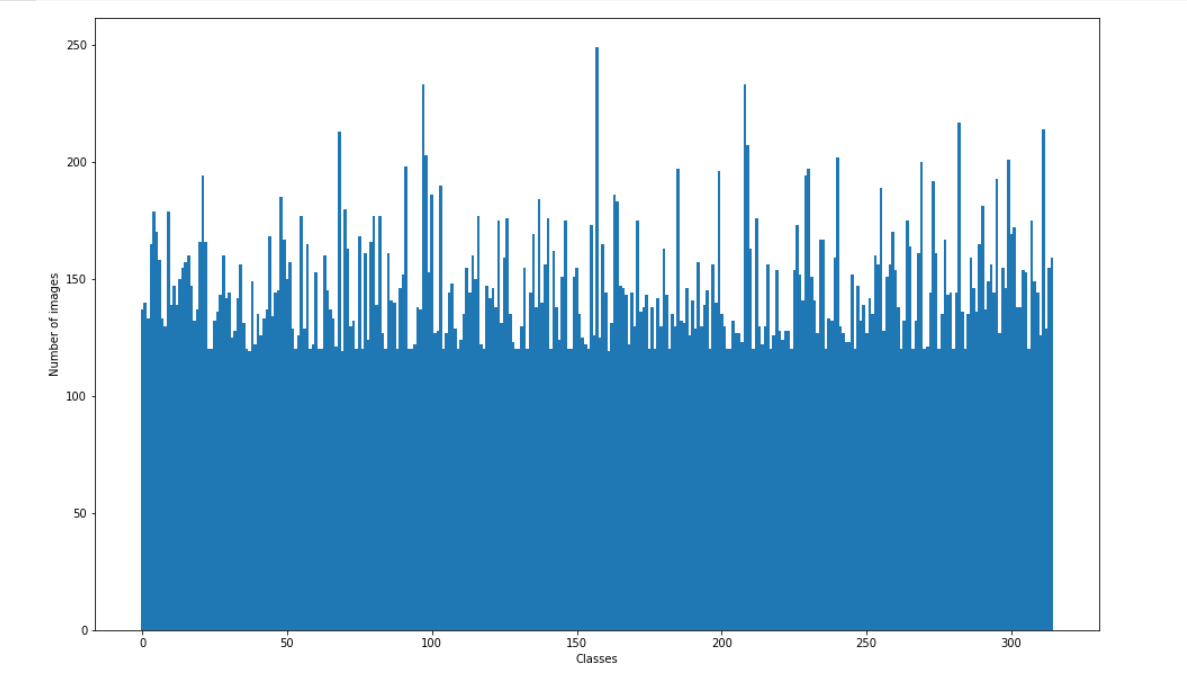
\includegraphics[width=\textwidth]{Figures/dataset distribution.png}
    \caption{Distribution of the number of images per label}
    \label{fig:ds_distribution}
\end{figure}

% Purposed Approach
\section{Purposed Approach}
\subsection{Convolutional Neural Network}
A Convolutional Neural Network (CNN) is a class of deep neural networks, most commonly applied to analyzing visual imagery. They have applications in image and video recognition, recommender systems, image classification, image segmentation, medical image analysis, natural language processing, brain-computer interfaces, and financial time series\cite{cnn_intro}. It was first proposed by Yan Lecun in 1998 for classifying handwriting number and now it is a widely applied deep neural network in the field of computer vision because of these some advantages. The CNN algorithm can avoid the explicit feature extraction, and implicitly to learn from the training data. CNN is also computationally efficient. It uses special convolution and pooling operations and performs parameter sharing. This enables CNN models to run on any device, making them universally attractive\cite{cnn_advan}.

\subsubsection{\large Theory}\hspace*{\fill} \\
All CNN models follow a similar architecture, which is shown in the figure below.
\begin{figure}[H]
    \centering
    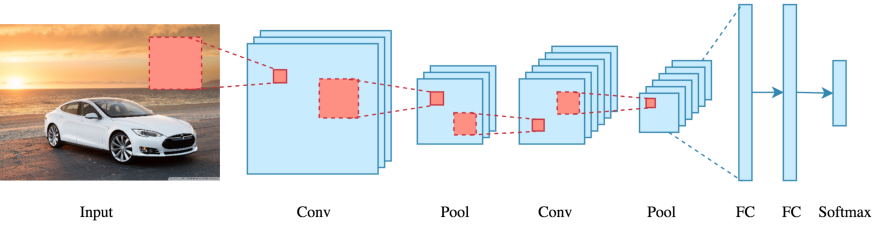
\includegraphics[width=\textwidth]{Figures/cnn.png}
    \caption{CNN architecture}
    \label{fig:cnn}
\end{figure}
As we can see, the CNN involves 3 main layers : Convolutional layer, Pooling layer and Fully Connected layer. We will now dive into each component.

\paragraph{\large\bf Convolutional layer}\hspace*{\fill} \\
Convolution layer is the first layer to extract features from images. Learnable parameters in this layer is a series of filters known as convolutional kernel. Kernel can be understood as a small 2D matrix of intergers with the size of k * k (k is an odd number and usually equal to 3, 5) which is used to establish a relationship of the center pixel with respect to its neighbor pixels. By sliding the kernel horizontally, vertically through the pixels in the images and performing \textbf{Convolution operation}, we can produce feature map which contains the extracted features of input images. When sliding kernel, we also need to care about \textbf{stride} and \textbf{padding}.
\vspace{2cm}

\paragraph{\bf Convolution operation}\hspace*{\fill} \\
Convolution is a mathematical operation to merge two sets of information. Given an input image $I$ and a filter (kernel) $K$ of dimensions $k_{1}, k_{2}$, the convolution operation is given by:

\begin{equation}
S(i, j)=(K * I)(i, j)=\sum_{m} \sum_{n} I(i-m, j-n) K(m, n)
\end{equation} 

\begin{figure}[H]
    \centering
    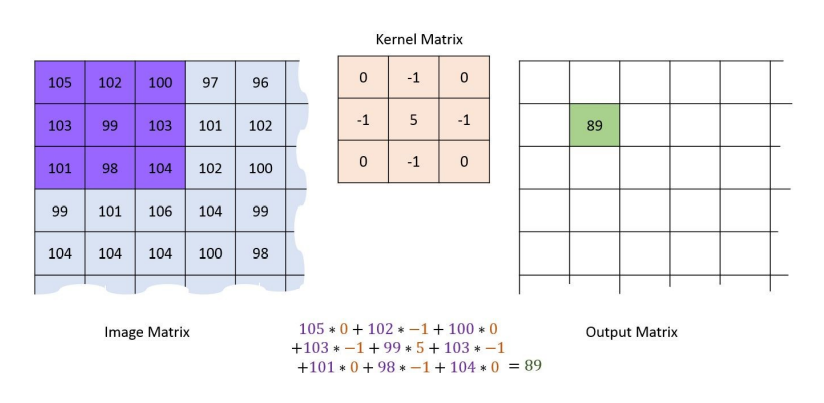
\includegraphics[width=0.7\textwidth]{Figures/convolution.png}
    \caption{Convolution operation }
    \label{fig:my_label}
\end{figure} 

\paragraph{\bf Stride}\hspace*{\fill} \\
Strides reflect the number of positions by which the kernel matrix shifts after applying a convolution on the middle element. A stride value of 1 indicates that the kernel matrix gets shifted only by 1 pixel in the either direction, right or down.\cite{cnn_project}
\begin{figure}[H]
    \centering
    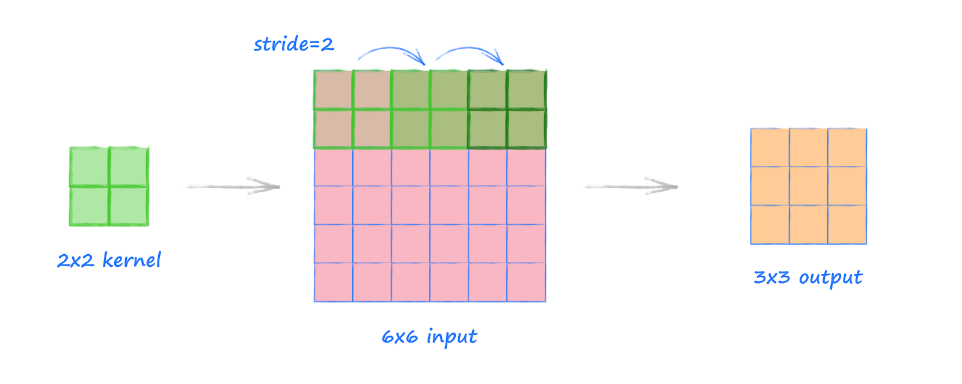
\includegraphics[width=0.7\textwidth]{Figures/stride.png}
    \caption{Affect of stride on movement of the kernel}
    \label{fig:stride}
\end{figure}

\paragraph{\bf Padding}\hspace*{\fill} \\
To conserve the information in edge pixels and keep the size of feature maps, we have to add a layer of zeros along the edges of the larger matrix/image. This addition of zeros on each side of the matrix is known as padding. If $N \times N$ is the dimension of the kernel matrix, we need to add $ \left\lfloor\frac{N}{2}\right\rfloor $ zero layers to the edges. \cite{cnn_project}

\begin{figure}[H]
    \centering
    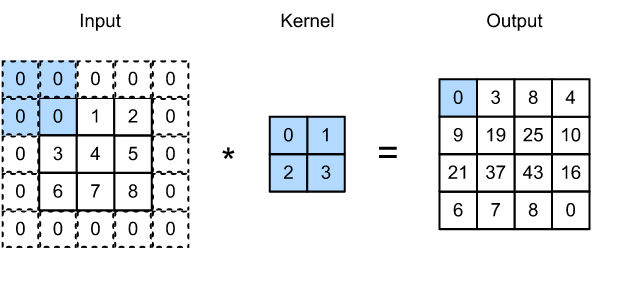
\includegraphics[width=10cm]{Figures/padding.png}
    \caption{Input and output when apply padding}
    \label{fig:padding}
\end{figure}

\paragraph{\large\bf Pooling layer}\hspace*{\fill} \\
Pooling layer is usually used between convolutional layers for reducing the spatial size but maintain important properties. The dimension reduction decrease the computational power required. In this process, rules of stride and padding are kept the same as above. There are three types of pooling: Max Pooling, Average Pooling and Global Pooling. In this project, I only use Max Pooling so that the output feature map contains the most prominent features of the previous feature map. Max Pooling is a pooling operation that selects the maximum element from the region of the feature map covered by the filter.

\begin{figure}[H]
    \centering
    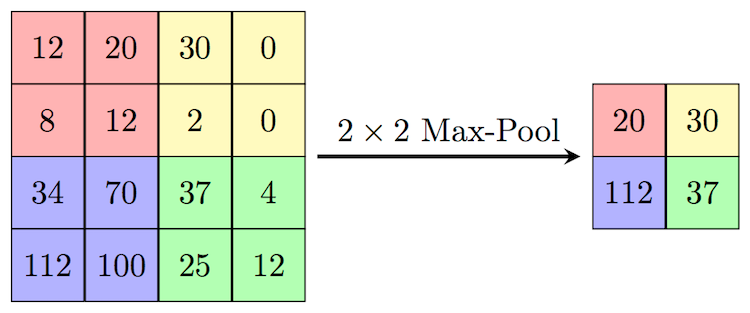
\includegraphics[scale=1.3]{Figures/pooling.png}
    \caption{Max Pooling}
    \label{fig:pooling}
\end{figure}

\paragraph{\large\bf Fully Connected Layer}\hspace*{\fill} \\
After the convolution + pooling layers we add a couple of fully connected layers to wrap up the CNN architecture. The fully connected layer has the same architecture as ANN and it can learn non-linear combinaions of the high-level features as represented by the output of the convolutional layer. Thus, it is usually used for classification task. The net input is calculated by an linear function:

\begin{equation}
N e t=w_{0} +\sum_{i=1}^{m} w_{i} x_{i}
\end{equation}

\begin{figure}[H]
    \centering
    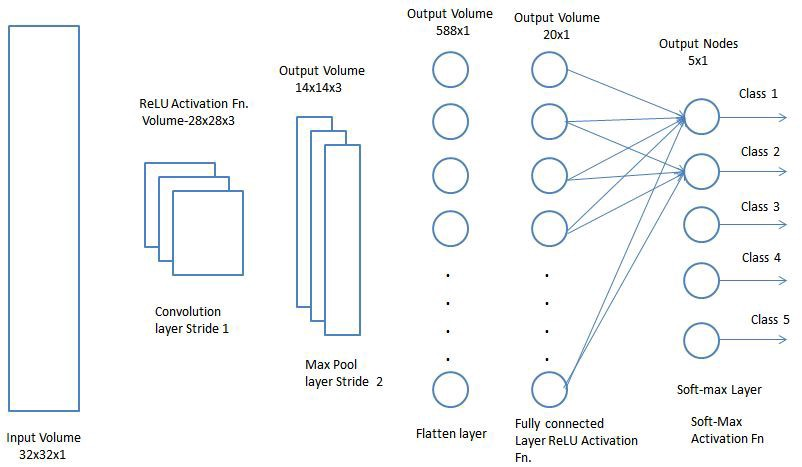
\includegraphics[width=10cm]{Figures/fc.jpeg}
    \caption{Fully Connected Layer}
    \label{fig:fc}
\end{figure}

\subsubsection{\large Network architecture}\hspace*{\fill} \\
As mention before, My Convolutional Neural Network model are built based on the architecture of AlexNet but with some adjustments. The architecture of the model are shown as below : 

\begin{figure}[H]
    \centering
    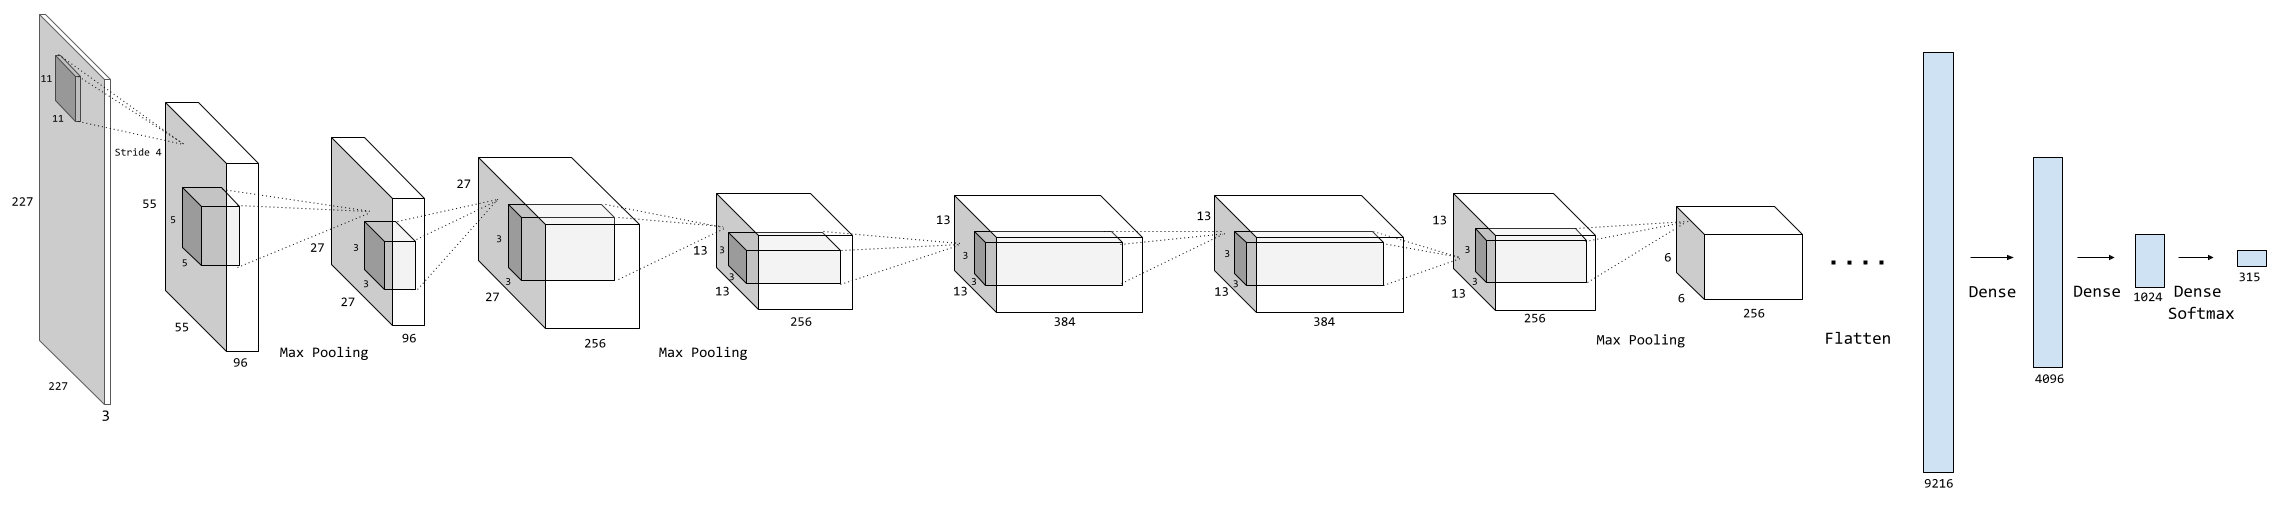
\includegraphics[width=\textwidth]{Figures/Model architecture.png}
\end{figure}
\begin{figure}[H]
    \centering
    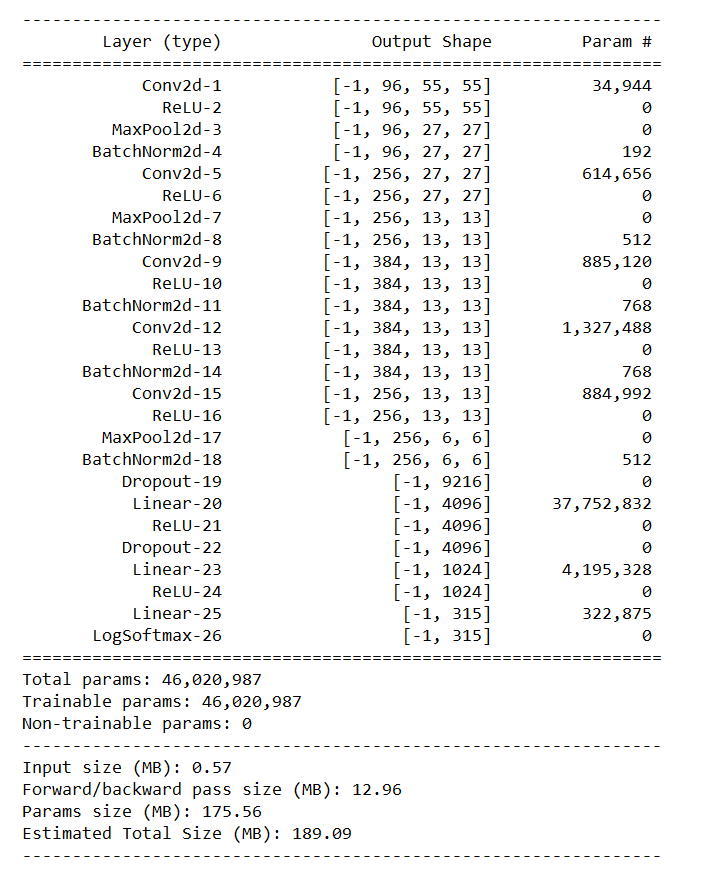
\includegraphics[width=10cm]{Figures/model summary.png}
    \caption{Network architecture and parameters}
    \label{fig:network}
\end{figure}
To decrease learning time and computational power, I added \textbf{Batch Normalization} layers in place of Local Response Normalization in AlexNet. I also add \textbf{Dropout} between fully connected layers in order to avoid overfitting. I used \textbf{ReLu function} as an activation function in all layers expect the last layer where I used \textbf{Softmax function} instead.

\paragraph{\large\bf Batch Normalization}\hspace*{\fill} \\
Batch normalization is a technique for training deep neural network that standardizes the inputs to a layer for each mini-batch. Batch normalization applies a transformation that maintains the mean output close to 0 and the output standard deviation close to 1. The input of batch norm layer are values of $x$ over a mini-batch: $ \mathcal{B}=\left\{x_{1 \ldots m}\right\} $. The Batch Normalization layer first determines the mean $\mu_{\mathcal{B}} = \frac{1}{m} \sum_{i=1}^{m} x_{i} $ and the variance $ \sigma_{\mathcal{B}}^{2} = \frac{1}{m} \sum_{i=1}^{m}\left(x_{i}-\mu_{\mathcal{B}}\right)^{2} $ of the activation values across the batch. It then normalizes the activation vector $ \widehat{x}_{i} = \frac{x_{i}-\mu_{\mathcal{B}}}{\sqrt{\sigma_{\mathcal{B}}^{2}+\epsilon}} $. That way, each neuron’s output follows a standard normal distribution across the batch. It finally calculates the layer’s output $ \hat{Z}_{i}$ by applying a linear transformation with this equation $ y_{i} = \gamma \widehat{x}_{i}+\beta \equiv \mathrm{BN}_{\gamma, \beta}\left(x_{i}\right) $ where $\gamma$ allows to adjust the standard deviation and $\beta$ allows to adjust the bias, shifting the curve on the right or on the left side, these two are learnable parameters\cite{bn}.

\begin{figure}[H]
    \centering
    \subfigure[]{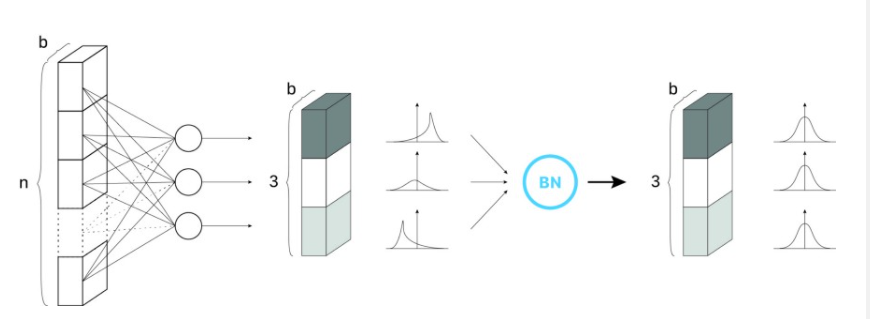
\includegraphics[width=0.5\textwidth]{Figures/bn.png}}
    \hspace{1cm}
    \subfigure[]{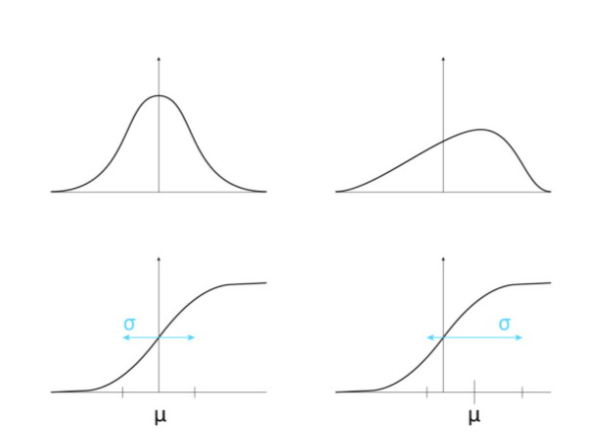
\includegraphics[width=0.3\textwidth]{Figures/y and b.png}}
    \caption{(a) Batch Normalization (b) Benefits of $\gamma$ and $\beta$}
    \label{fig:bn}
\end{figure}

\paragraph{\large\bf Dropout}\hspace*{\fill} \\
Dropout is a technique where randomly selected neurons are ignored during training. They are “dropped-out” randomly. This means that their contribution to the activation of downstream neurons is temporally removed on the forward pass and any weight updates are not applied to the neuron on the backward pass.\cite{cnn_project}

\begin{figure}[H]
    \centering
    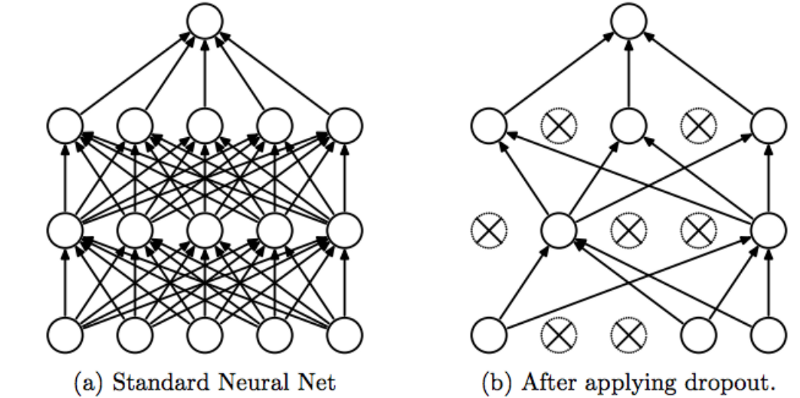
\includegraphics[width=10cm]{Figures/dropout.png}
    \label{fig:dropout}
\end{figure}

\paragraph{\large\bf Activation function}\hspace*{\fill}
\paragraph{\bf Relu}\hspace*{\fill} \\
The ReLU is the most used activation function in the world right now. The ReLU function and its derivative are both monotonic, which makes it efficient and easy for computation. The ReLU function is shown below:

\begin{equation}
\begin{aligned}
    &Equation: f(x) = max(0, x) \\
    &Range: 0 \rightarrow \inf
\end{aligned}
\end{equation}

\paragraph{\bf Softmax}\hspace*{\fill} \\
The softmax function is also a type of sigmoid function but it is very useful to handle classification problems having multiple classes. 
\begin{equation}
\sigma(z)_{j}=\frac{e^{z_{j}}}{\sum_{k=1}^{K} e^{z_{k}}}
\end{equation}
The softmax function is shown above, where $z$ is a vector of the inputs to the output layer (if you have 10 output units, then there are 10 elements in $z$). And again, j indexes the output units, so $j = 1, 2, ..., K$. The softmax function is ideally used in the output layer of the classifier where we are trying to attain the probabilities to define the class of each input\cite{cnn_project}. So I use that in output layer for classification task.

\subsubsection{Training}\hspace*{\fill} \\
I trained the model on my training dataset. I measured the error of my model by calculating \textbf{Cross Entropy Loss} between predicted value and actural value. To get predicted value, I forwarded the data through the network and then calculated loss at each layer by using a technique called \textbf{backward propagation}. And finally, I use \textbf{Adam Optimization algorithm} to update the parameters of the model.

\paragraph{\large\bf Cross Entropy Loss}\hspace*{\fill} \\
Cross Entropy Loss evaluates the performance of a classification model whose output represents the probability which label are true label, its value is between 0 and 1. Cross Entropy Loss increases when the predicted probability diverges from the actural label. In binary classification, Cross Entropy can be calculated as :
\begin{equation}
-(y \log (p)+(1-y) \log (1-p))
\end{equation}

In multiclass classification, we calculate the loss separately for each label and sum the result:
\begin{equation}
E = -\sum_{c=1}^{M} y_{o, c} \log \left(p_{o, c}\right)
\end{equation}

\noindent    Where : \\
$M$ - number of classes \\
$y$ - binary indicator if class label $c$ is correct for observation $o$ \\
$p$ - predicted probability observation $o$ is of class $c$ 

\paragraph{\large\bf Adam Optimization algorithm}\hspace*{\fill} \\
Adam Optimization algorithm can be looked at as a combination of RMSprop and Stochastic Gradient Descent with momentum. It uses the gradients to scale the learning rate like RMSprop and it takes advantage of momentum by using moving average of the gradient instead of gradient itself like SGD with momentum\cite{adam}.

\paragraph{\large\bf Backward Propagation}\hspace*{\fill} \\
In order to update the parameters, we need to calculate gradients of the error. In convolutional layer, we have to compute 2 things : the derivative of error with respect to the trainable parameters of the kernels, biases and the derivative of error with respect to the input of the layer so that the previous layer can take it as the derivative of error with respect to its own output and perform the same operations. It is calculated by apply these 3 equation : 
\begin{equation}
\begin{aligned}
\frac{\partial E}{\partial K_{i j}} &=X_{j} \star \frac{\partial E}{\partial Y_{i}} \\
\frac{\partial E}{\partial B_{i}} &=\frac{\partial E}{\partial Y_{i}} \\
\frac{\partial E}{\partial X_{j}} &=\sum_{i=1}^{n} \frac{\partial E}{\partial Y_{i}} *_{f u l l}^{*} K_{i j}
\end{aligned}
\end{equation}
Where : \\
E - Error signal \\ 
$K_{i j}$ - Parameters $k$ in row $i$ and column $j$ of the kernel $K$ \\
$X_{j}$ - Column $j$ of the input matrix $X$ \\ 
$Y_{i}$ - Row $i$ of the output matrix $Y$ \\ 
$B_{i}$ - Row $i$ of the bias matrix $B$ 

\subsection{Transfer Learning}
Transfer learning is a machine learning technique of reusing a developed model for a task for a model on an other task. It is a popular approach in deep learning where pre-trained models which were trained with a big dataset, given a vast compute power and time resources are used as the starting point on related problems so that it can learn more quickly and perform properly.\\
In this project, I used ResNet18 as the backbone and I only change the last fully connected layer for classification task.

\subsection{Image Retrieval}
An image retrieval system is a computer system used for browsing, searching and retrieving images from a large database of digital images.\cite{ir} To solve the bird classification problem, first I need a method to vectorize the input images and build a gallery of vertorized image. Then to predict the label of query image, I vectorize it and find the k most similar vector in the dataset. In this project, I used pre-trained ResNet18 with the absence of last fully connected layer as a vectorization model and I calculated the \textbf{Euclidean distance} between query vector and every vectors in the gallery to get the similarity between the vectors. Finally, I take the k closest vector to the query vector and get the dominant label as the predicted label for query image. The procedure of the method is shown in the picture: 
\begin{figure}
    \centering
    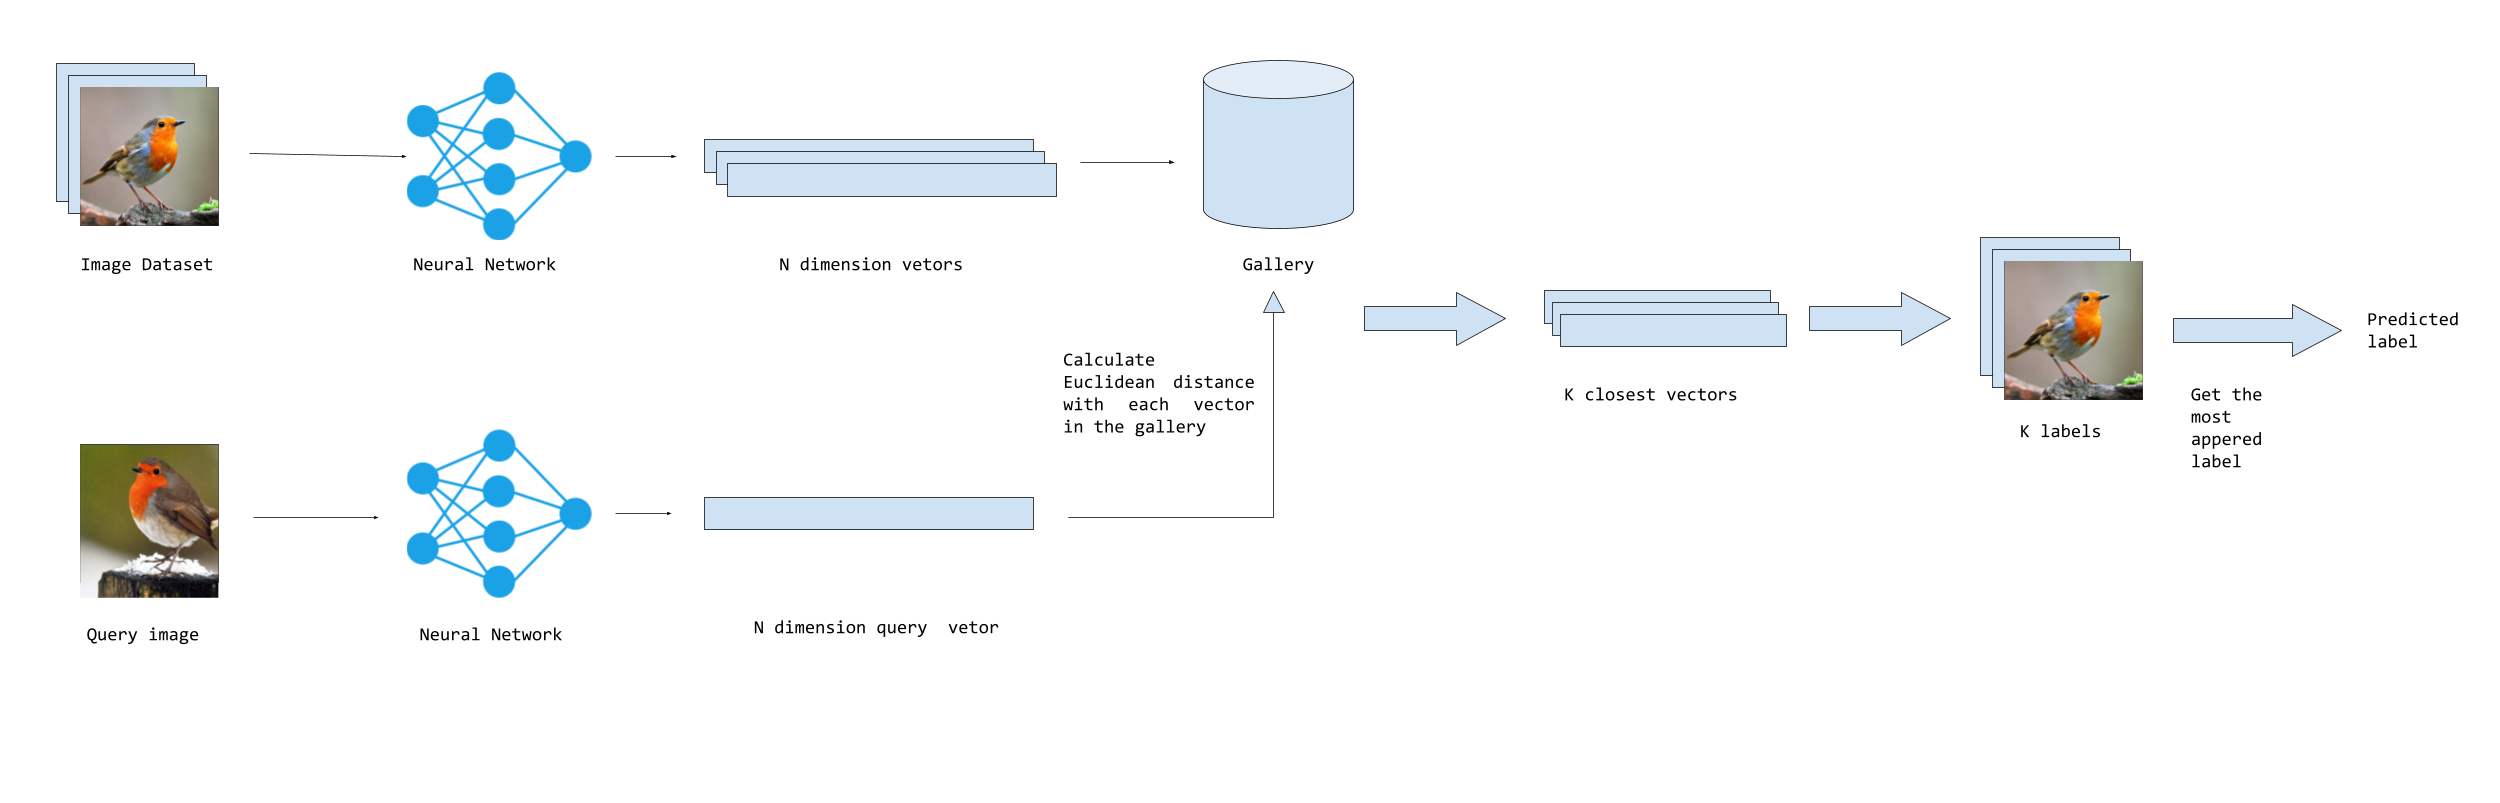
\includegraphics[width=\textwidth]{Figures/Image retrieval.png}
    \caption{Image Retrieval method procedure}
    \label{fig:image retri}
\end{figure}

\paragraph{\large\bf Euclidean Distance}\hspace*{\fill} \\
The distance between 2 n-dimension vectors is calculated by this equation :
\begin{equation}
Euclidean Distance = d(x, y) =\sqrt{\sum_{k=1}^{n}\left(x_{k}-y_{k}\right)^{2}}
\end{equation}

\section{Training}
\paragraph{\large\bf Technology and Frameworks used}\hspace*{\fill} \\
Progamming Language : Python 3.9\\
Used Frameworks and Python packages : numpy, matplotlib, pandas, pytorch, torchvision, tensorboard, tqdm, jupyter, PIL, pickle\\
Environment: Google Colaboratory vitural machine
\paragraph{\large\bf Hardware}\hspace*{\fill} \\
I trained my model on Google Colaboratory vitural machine with Tesla K80 GPU for free user. 
\paragraph{\large\bf Training technique}\hspace*{\fill} \\
To avoid overfitting, I reduce learning rate if the evaluation results on validation set weren't better after 2 epochs. In addition, I trained my network in batch with the batch size of 1024 to accelerate training process.
\paragraph{\large\bf Training process}\hspace*{\fill} 
\paragraph{\bf Scratch Model} 
With my scratch CNN model, I trained it for 30 epochs. It cost about 3600s to train some first epochs and then decreased to about 2700s per epoch. Loss in training and validation accuracy are shown in the graphs below :
\begin{figure}[H]
    \centering
    \subfigure[]{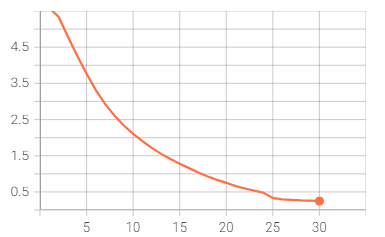
\includegraphics[width=0.33\textwidth]{Figures/Scratch_train.png}}
    \subfigure[]{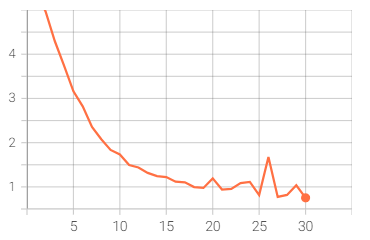
\includegraphics[width=0.33\textwidth]{Figures/Scratch_val_loss.png}}
    \subfigure[]{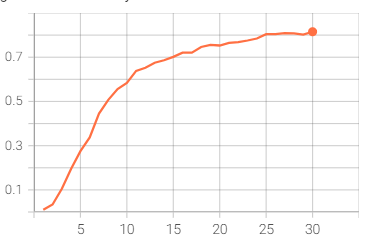
\includegraphics[width=0.33\textwidth]{Figures/Scratch_val_acc.png}}
    \caption{(a) Training loss (b) Validation loss (c) Validation accuracy}
    \label{fig:scratch}
\end{figure}
\paragraph{\bf Transfer Learning} 
By using transfer learning, I retrained the ResNet18 model for 2 versions: for version 1, I freezed all convolutional layer and only trained the last fully connected layer; for version 2, I retrained all the network. The time consumption for training these 2 version is 3600s for the first epoch and about 360s for others. The loss of the network converged after 10 epochs of training but the loss of version 2 wasn't stable. Loss in training and validation accuracy are shown in the graphs below :
\begin{figure}[H]
    \centering
    \subfigure[]{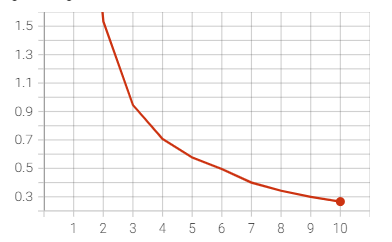
\includegraphics[width=0.32\textwidth]{Figures/Resnet_TL.png}}
    \subfigure[]{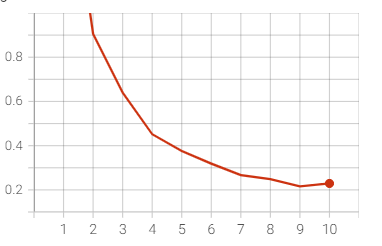
\includegraphics[width=0.32\textwidth]{Figures/Resnet_TL_Valloss.png}}
    \subfigure[]{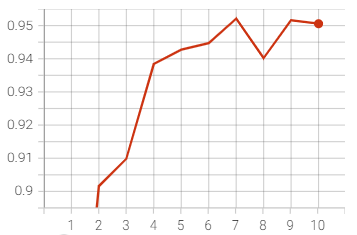
\includegraphics[width=0.32\textwidth]{Figures/Resnet_TL_Valacc.png}}
    \caption{ResNet Transfer Learning version 1 (a) Training loss (b) Validation loss (c) Validation accuracy}
    \label{fig:resnet1}
\end{figure}
\begin{figure}[H]
    \centering
    \subfigure[]{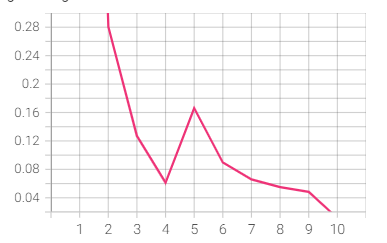
\includegraphics[width=0.33\textwidth]{Figures/Resnet_TL_Full_train.png}}
    \subfigure[]{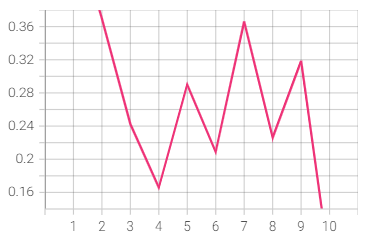
\includegraphics[width=0.33\textwidth]{Figures/Resnet_TL_Full_val_loss.png}}
    \subfigure[]{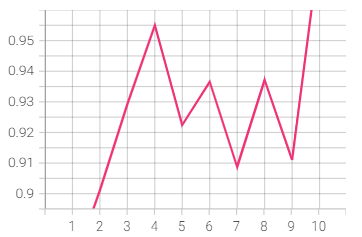
\includegraphics[width=0.33\textwidth]{Figures/Resnet_TL_Full_val_acc.png}}
    \caption{ResNet Transfer Learning version 2 (a) Training loss (b) Validation loss (c) Validation accuracy}
    \label{fig:resnet2}
\end{figure}
\paragraph{\bf Image Retrieval} 
To build the gallery for image retrieval, I used the second version of ResNet18 trained above. For saving memory, reducing predict time and solving unbalance data problem, I limited the number of images in my gallery to 50 images per label for 315 bird species. In total, there are 15750 vectors of images in my gallery. The time cost to build gallery is about 22 minutes.
\section{Results and evaluation}
In this project, I used 3 evaluation method to measure my model performance.
\paragraph{\large\bf Exact Match Ratio}\hspace*{\fill} \\
The Exact Match Ratio is defined as :
\begin{equation}
   \textit{Exact Match Ratio} = \frac{\textit{Number of examples with exact label match}}{\textit{Total number of examples}}
\end{equation}
\vspace{3cm}
\paragraph{\large\bf Classification Report}\hspace*{\fill} \\
In classification report, there are 3 evaluation metrics we need to care: \\
1. Precision: It is the ratio of correctly predicted positive observations to the
total observations. It is defined as:
\begin{equation}
    \frac{TruePositives}{TruePositives + FalsePositives}
\end{equation}
2. Recall: It is the ratio of correctly predicted positive observations to all the
observations in the relevant class.
\begin{equation}
    \frac{TruePositives}{TruePositives + FalseNegatives}
\end{equation}
3. F1-score: It is the harmonic mean of precision and recall.\cite{cnn_project}
\begin{equation}
    2 * \frac{precision * recall}{precision + recall}
\end{equation}
Because of large number of labels in this dataset, I only cared about the average precision, recall and f-1 score.
\paragraph{\large\bf Confusion Matrix}\hspace*{\fill} \\
The confusion matrix shows the ways in which your classification model is confused when it makes predictions. It gives you insight not only into the errors being made by your classifier but more importantly the types of errors that are being made.

\subsection{\large\bf Scratch Model}
With my scratch model, it can guess 82\% correct images in testing dataset. The testing result and confusion matrix are shown in the pictures below.
\begin{figure}[H]
    \centering
    \subfigure[]{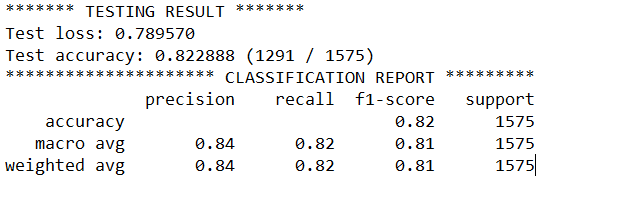
\includegraphics[width=0.7\textwidth]{Figures/scratch_result.png}}
    \subfigure[]{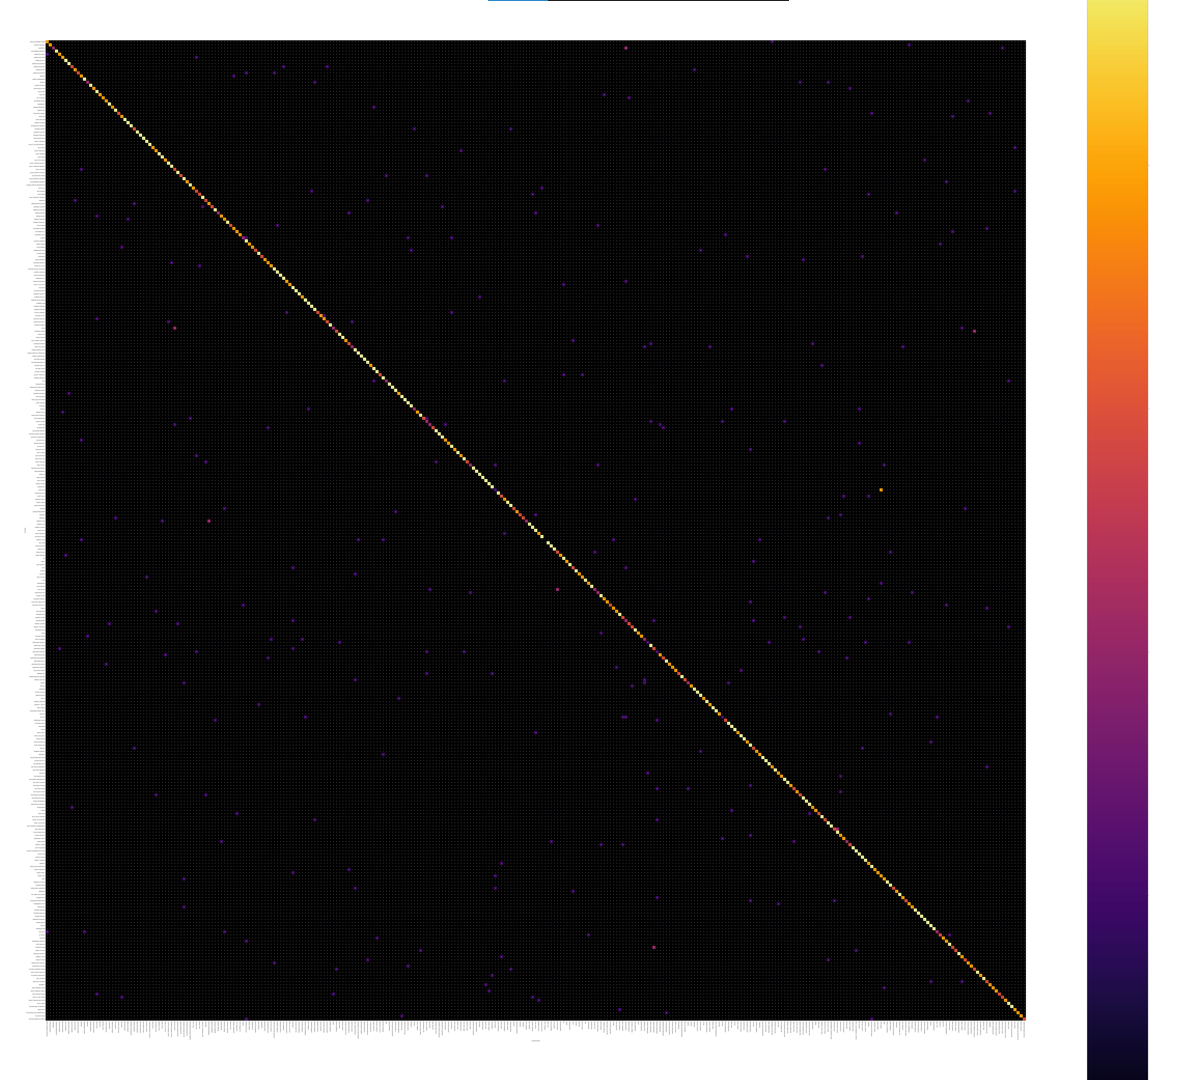
\includegraphics[width=0.8\textwidth]{Figures/alexnet_scratch.png}}
    \caption{(a) Testing result (b) Confusion matrix}
    \label{fig:sc_test}
\end{figure}
\subsection{\large\bf Transfer Learning model}
After testing, I can see that the ResNet that I retrained all the convolutional layer performs better than the ResNet version that I only trained the last fully connected layer. The testing result and confusion matrix are shown in the pictures below.
\begin{figure}[H]
    \centering
    \subfigure[]{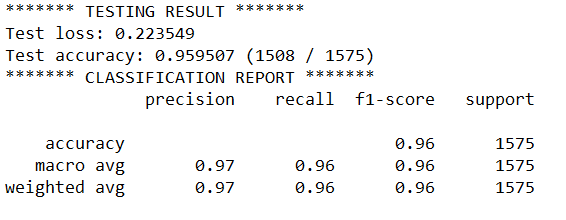
\includegraphics[width=0.7\textwidth]{Figures/res1_result.png}}
    \subfigure[]{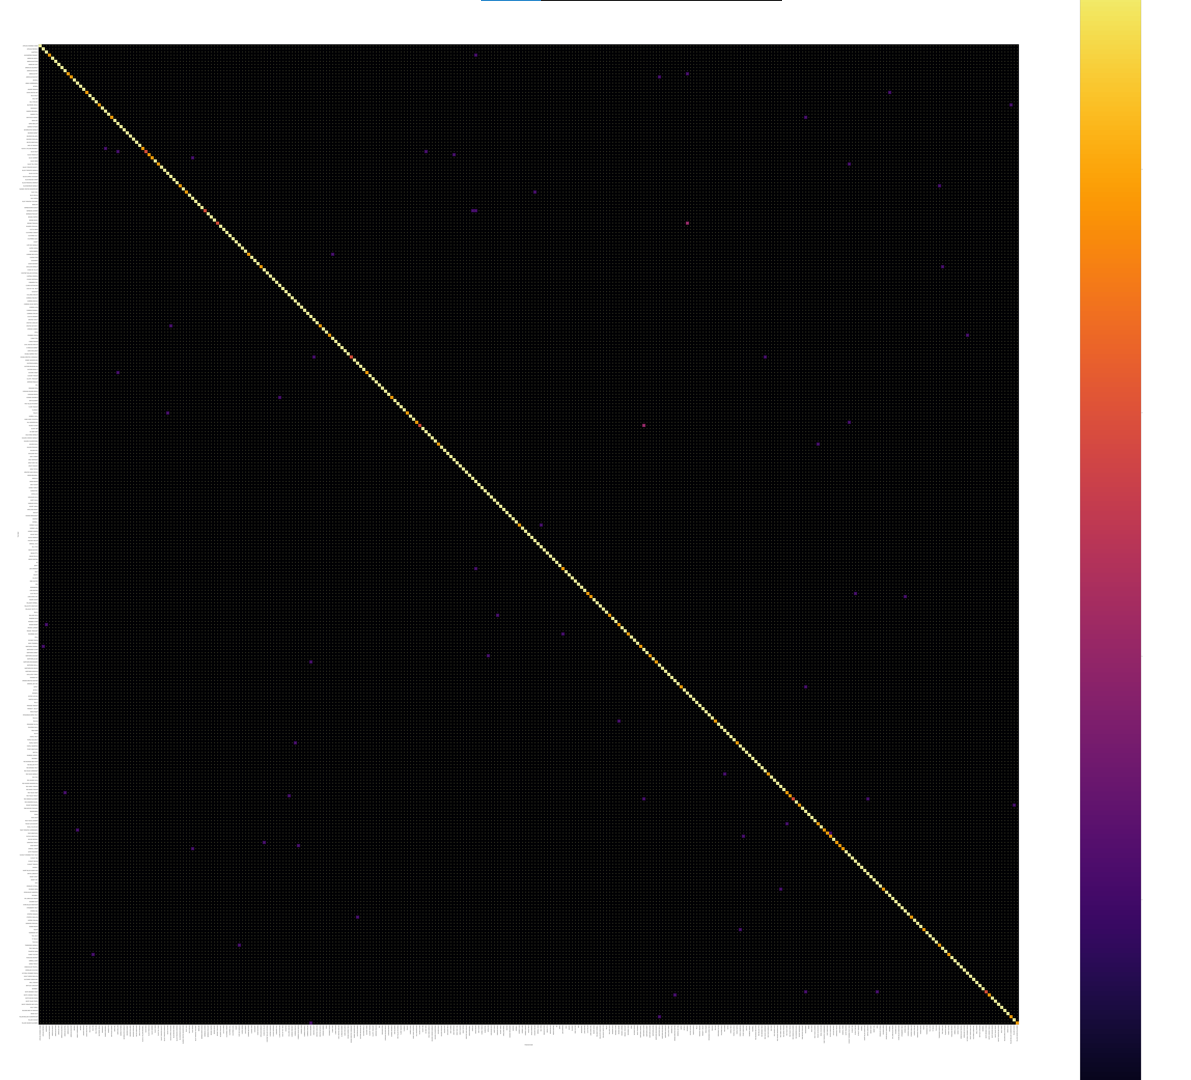
\includegraphics[width=0.8\textwidth]{Figures/res1_cm.png}}
    \caption{(a) Testing result (b) Confusion matrix of Transfer ResNet only trained last fully connected layer}
    \label{fig:rn1_test}
\end{figure}
\begin{figure}[H]
    \centering
    \subfigure[]{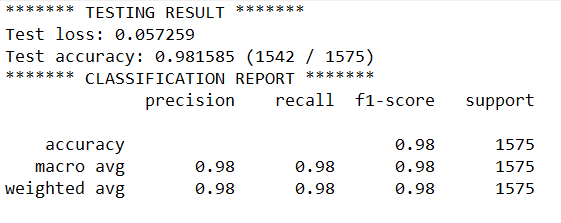
\includegraphics[width=0.7\textwidth]{Figures/res2_result.png}}
    \subfigure[]{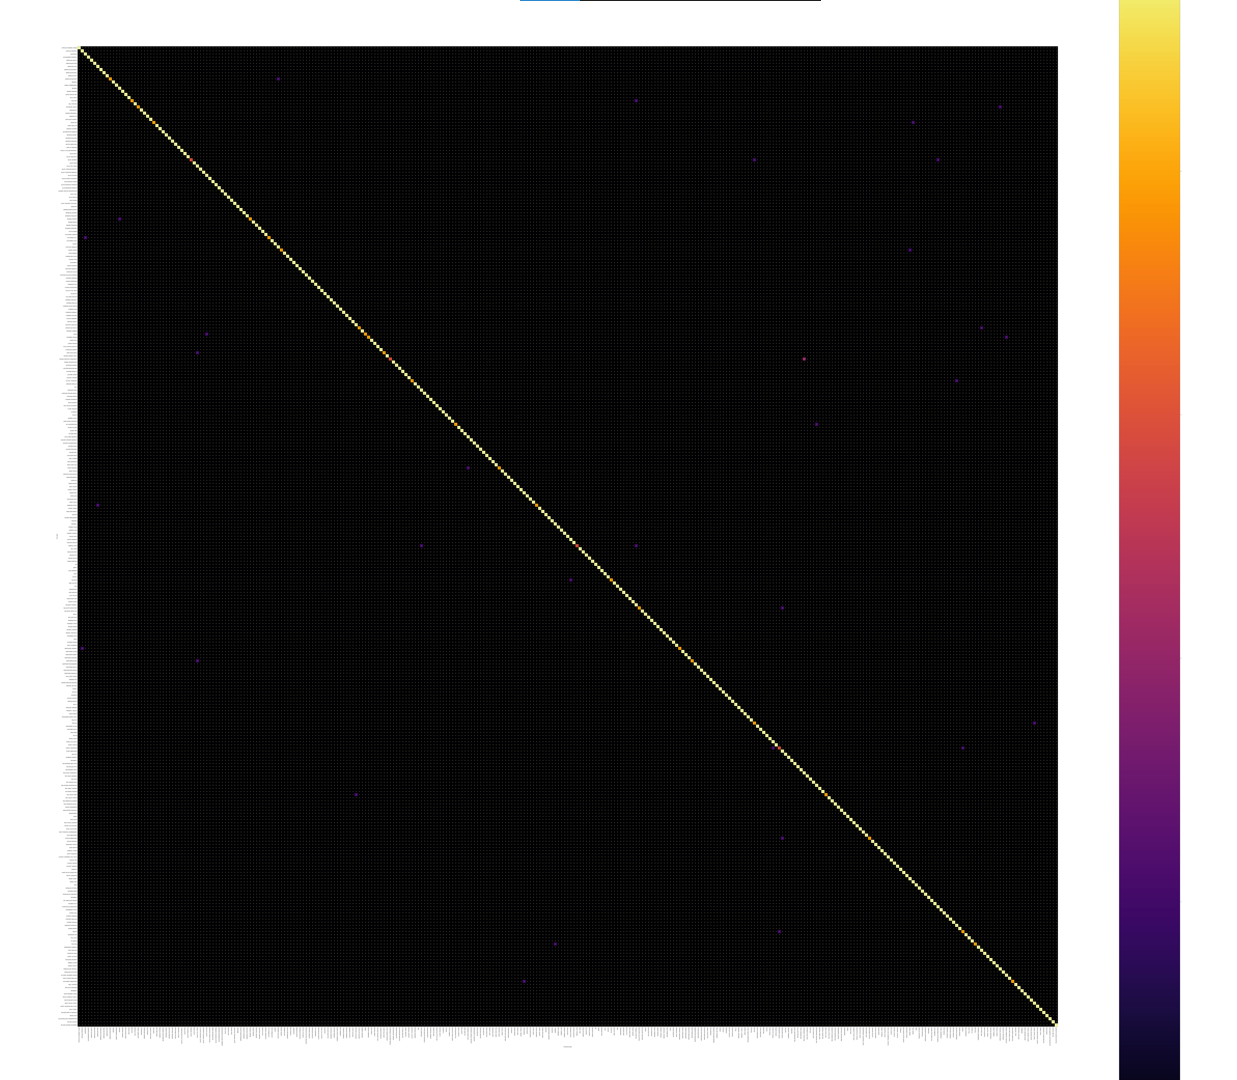
\includegraphics[width=0.8\textwidth]{Figures/res2_cm.png}}
    \caption{(a) Testing result (b) Confusion matrix of Transfer ResNet retrained all the network}
    \label{fig:rn2_test}
\end{figure}
\subsection{\large\bf Image Retrieval}
In this method, I set my k which is the hyper parameter of selecting k most similar vectors to query vector for getting prediction equal to 5. The pictures below displays how my system shows 9 most similar images to query image and evaluation result.

\begin{figure}[H]
    \centering
    \subfigure[]{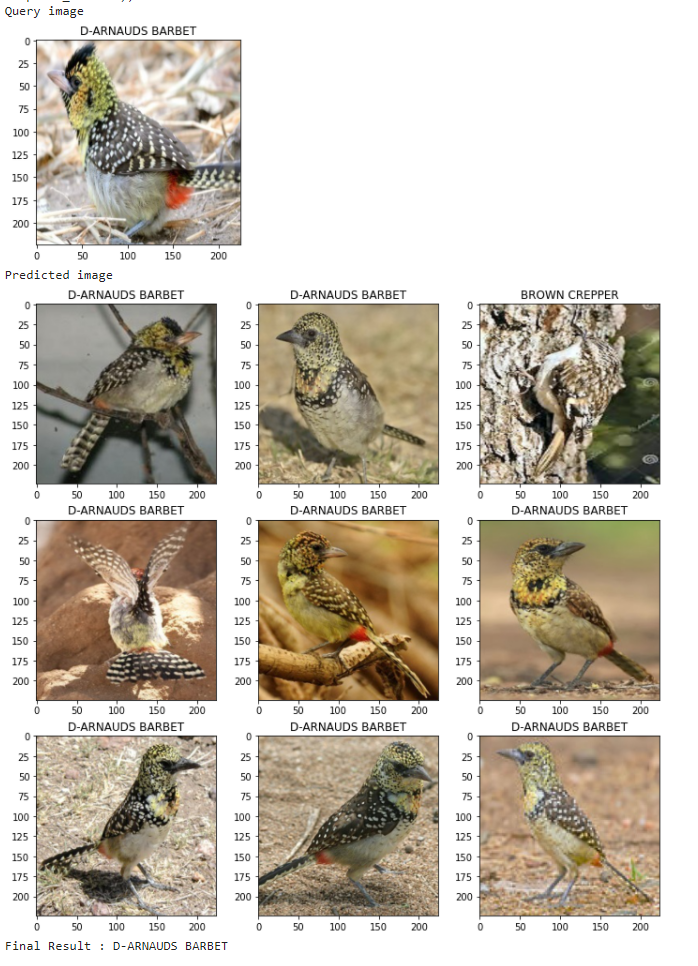
\includegraphics[width=0.3\textwidth]{Figures/ir.png}}
    \hspace{2cm}
    \subfigure[]{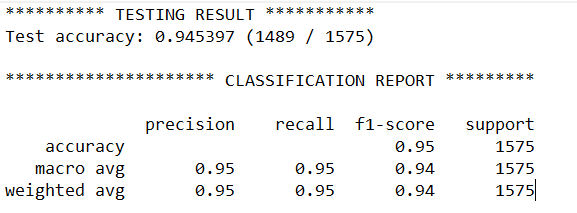
\includegraphics[width=0.5\textwidth]{Figures/ir-test.png}}
    \subfigure[]{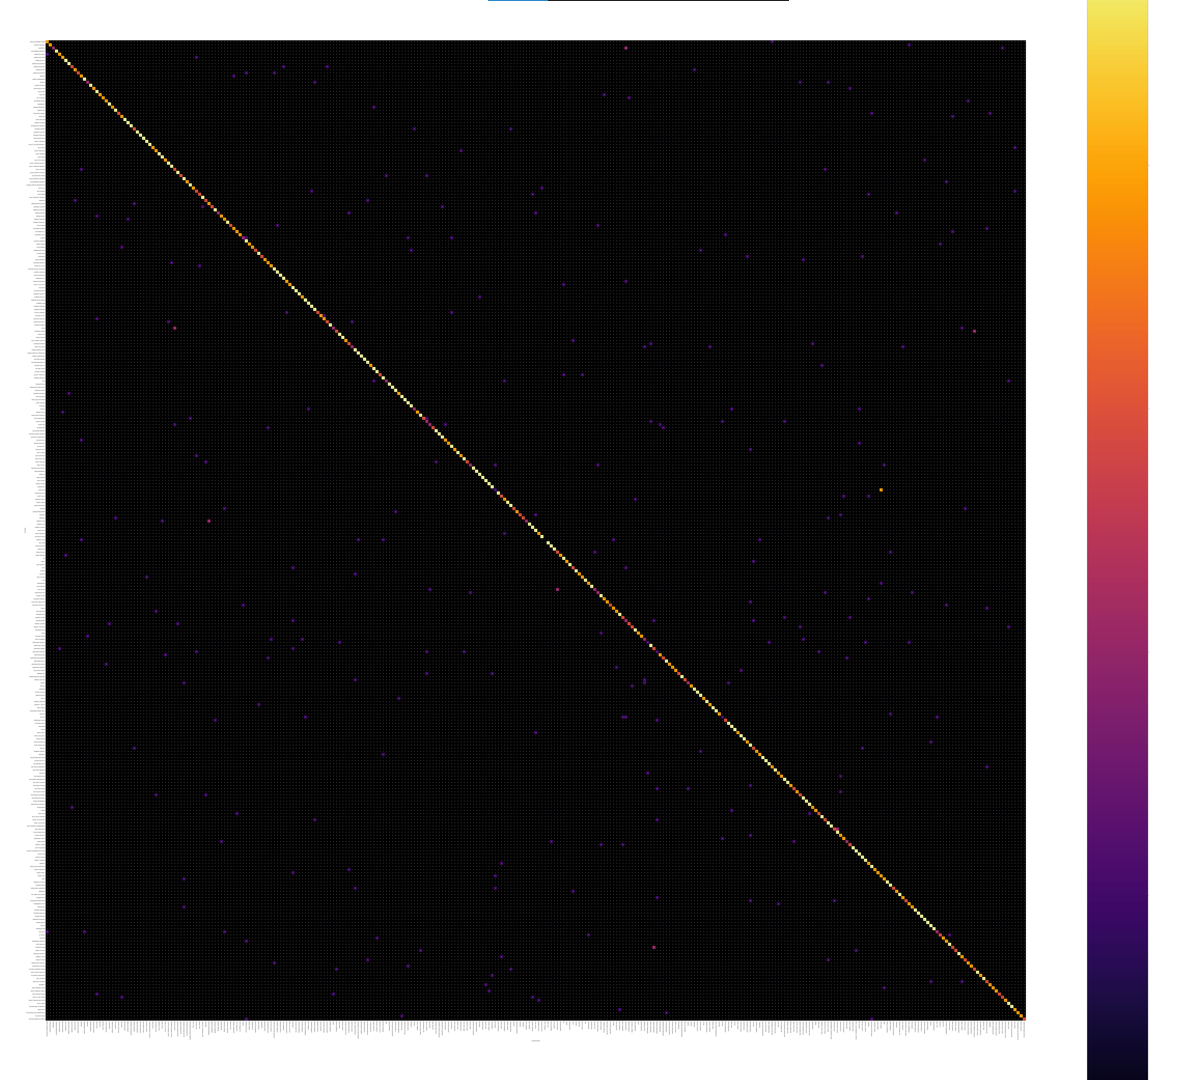
\includegraphics[width=0.8\textwidth]{Figures/alexnet_scratch.png}}
    \caption{(a) Get retrieve images (b) Testing result (c) Confusion matrix}
    \label{fig:ir_test}
\end{figure}
\section{Conclusion}
In this project, I have proposed 3 method to classify the species of the bird from high-definition camera photos by using CNN, transfer learning and image retrieval. The testing result shows that the model using transfer learning achieved the highest overall F1 score equal to 98$\%$. In the end, this project can help researcher easily identify known birds and contribute to bird preservation by arousing people interest of bird. However, my system not yet have a user interface, which can be hard to upload a photo of bird and get the name of the species. Besides, this model have only trained for 315 of bird species whereas there are thousand of bird types out there. I need to update frequently to get in keep to the various change in bird categories.\\
Through this project, I have learned how to solve a basic computer vision problem which is image classification problem. I know how to use CNN, transfer learning and the method to find an image in a big dataset. 
\section{Future work}
\noindent 1) Find a way to solve the unbalance data problem.\\
2) Apply basic Computer Vision technique such as filter, Object Detection, Segmentation for the model to work well on a hard or bad photographs.\\
3) Build UX/UI so user can easily access and use the system.

\printbibliography
\end{document}